% INTRODUCCIÓN

\cleardoublepage

\chapter{Sistema RAG aplicado a la Constitución Española}

\section{Introducción}

En este capítulo se presenta un caso práctico de laboratorio en el que se diseña un sistema RAG orientado a la recuperación de información de la Constitución Española para responder preguntas relacionadas con dicho documento.

El contenido de este capítulo incluye una justificación de los modelos empleados en el proceso, un análisis detallado del documento (Constitución Española), la definición de las estrategias de chunkerización utilizadas, justificación mediante métricas de la estrategia escogida, y finalmente, la implementación del agente capaz de responder a preguntas sobre el documento.

Todo el código referente a este capítulo se encuentra en el github \url{https://github.com/drumalv/tfm/tree/main/code}.


\section{Modelos usados}

Para el sistema RAG creado han sido necesarios 3 modelos. Por simplicidad para el hardware necesario se van a usar los modelos via API. Para este trabajo se usará la nube de Microsoft Azure y el recurso Azure OpenAI sobre el que se consumirán mediante API los modelos a continuación mencionados.

\subsection{Modelo Juez}

Modelo LLM encargado de evaluar las respuestas aportadas por el agente. Para esta tarea es necesario un modelo con alta calidad y razonamiento en sus respuestas.

En este caso se ha usado el modelo GPT-4o debido a que en el momento de la creación de este trabajo era el modelo más capaz según todos los benchmarks como puede verse en la figura \ref{fig:benchmark} (no tiene puntuación en Chatbot Arena debido a que no ha sido evaluado en esa métrica). Como otros puntos fuertes podemos ver en la figura \ref{fig:pricing} que tiene un precio contenido con respecto a sus competidores directos en calidad y además como se ve en la figura \ref{fig:speed} es más rápido en sus respuestas.

Finalmente, la característica clave para su elección es la relación calidad/precio donde en el momento de el desarrollo de este trabajo no tenía rival (véase la figura \ref{fig:quality_price}).


\subsection{Modelo del Agente}

Modelo LLM encargado de dar respuesta a una pregunta en base al contexto aportado. Este modelo no es necesario que sea de la calidad del modelo anterior ya que es de suponer que tendrá el contexto suficiente para resolver la pregunta del usuario.

Para el modelo del agente se ha elegido GPT-3.5-Turbo ya que muestra la mejor relación velocidad/precio. Hay que tener en cuenta que este modelo será el que podrá ser consultado en masa para responder preguntas sobre la constitución española y por tanto tanto la velocidad de respuesta como el precio forman un valor diferencial (véase las figuras \ref{fig:pricing} y \ref{fig:speed}.


\begin{figure}[h]
\centering
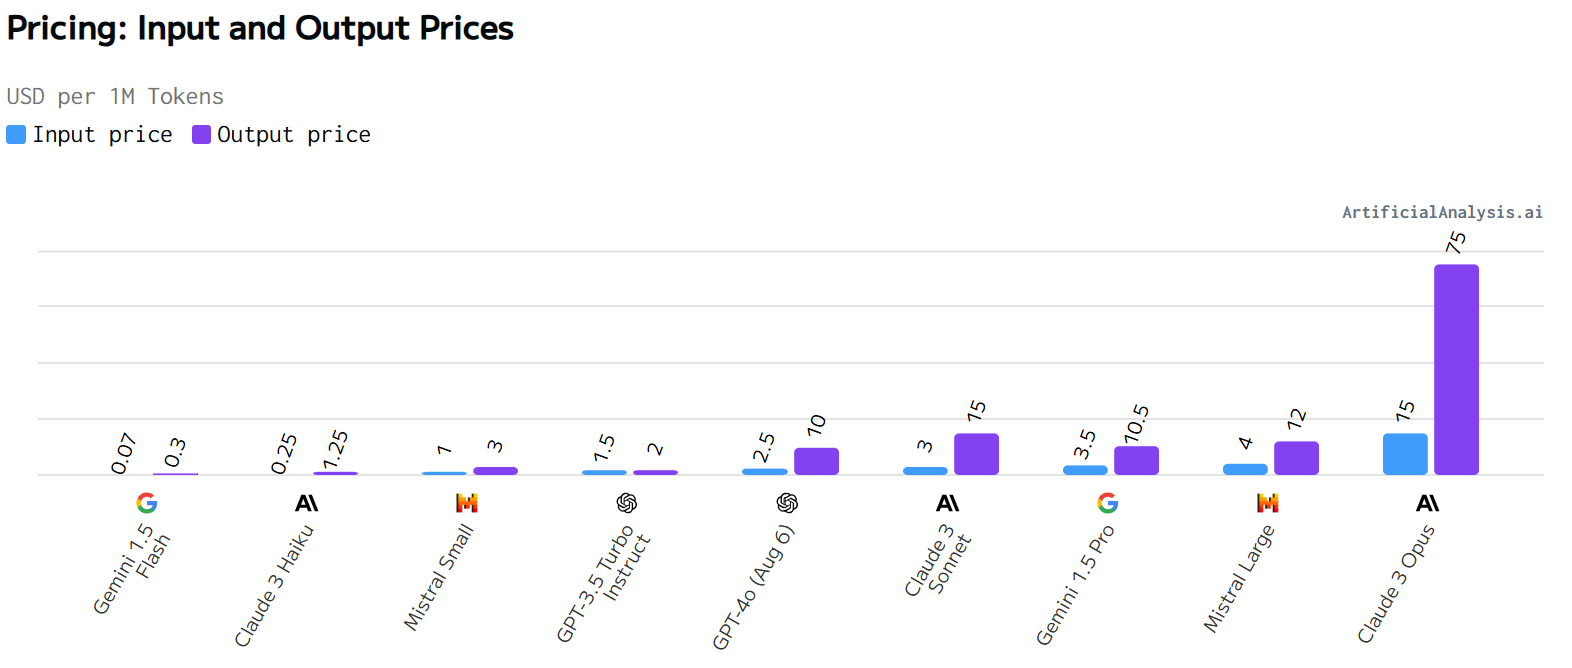
\includegraphics[width=0.9\textwidth]{figuras/capitulo6/pricing.png}
\caption{Benchmark sobre el precio de los LLMs evaluados. \citep{artificialanalysis}}
\label{fig:pricing}
\end{figure}

\begin{figure}[h]
\centering
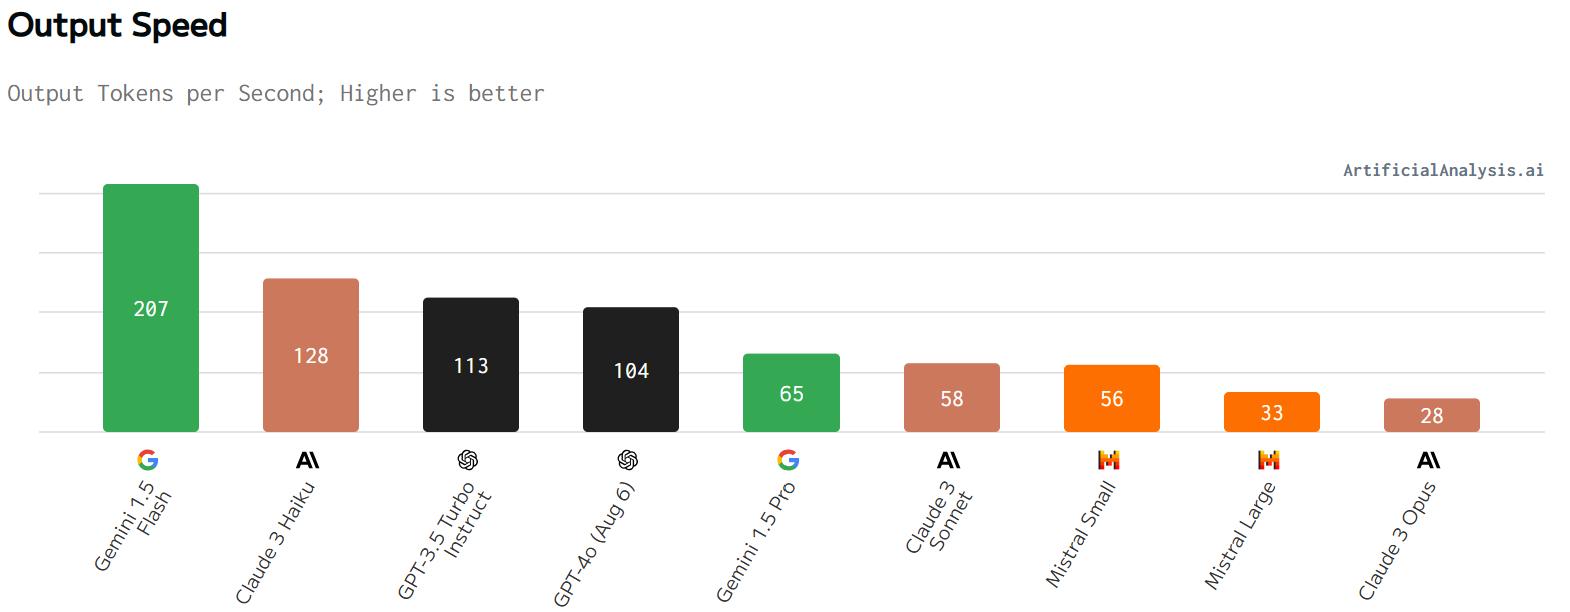
\includegraphics[width=0.9\textwidth]{figuras/capitulo6/speed.png}
\caption{Benchmark sobre la velocidad de respuesta de los LLMs evaluados. \citep{artificialanalysis}}
\label{fig:speed}
\end{figure}

\begin{figure}[]
\centering
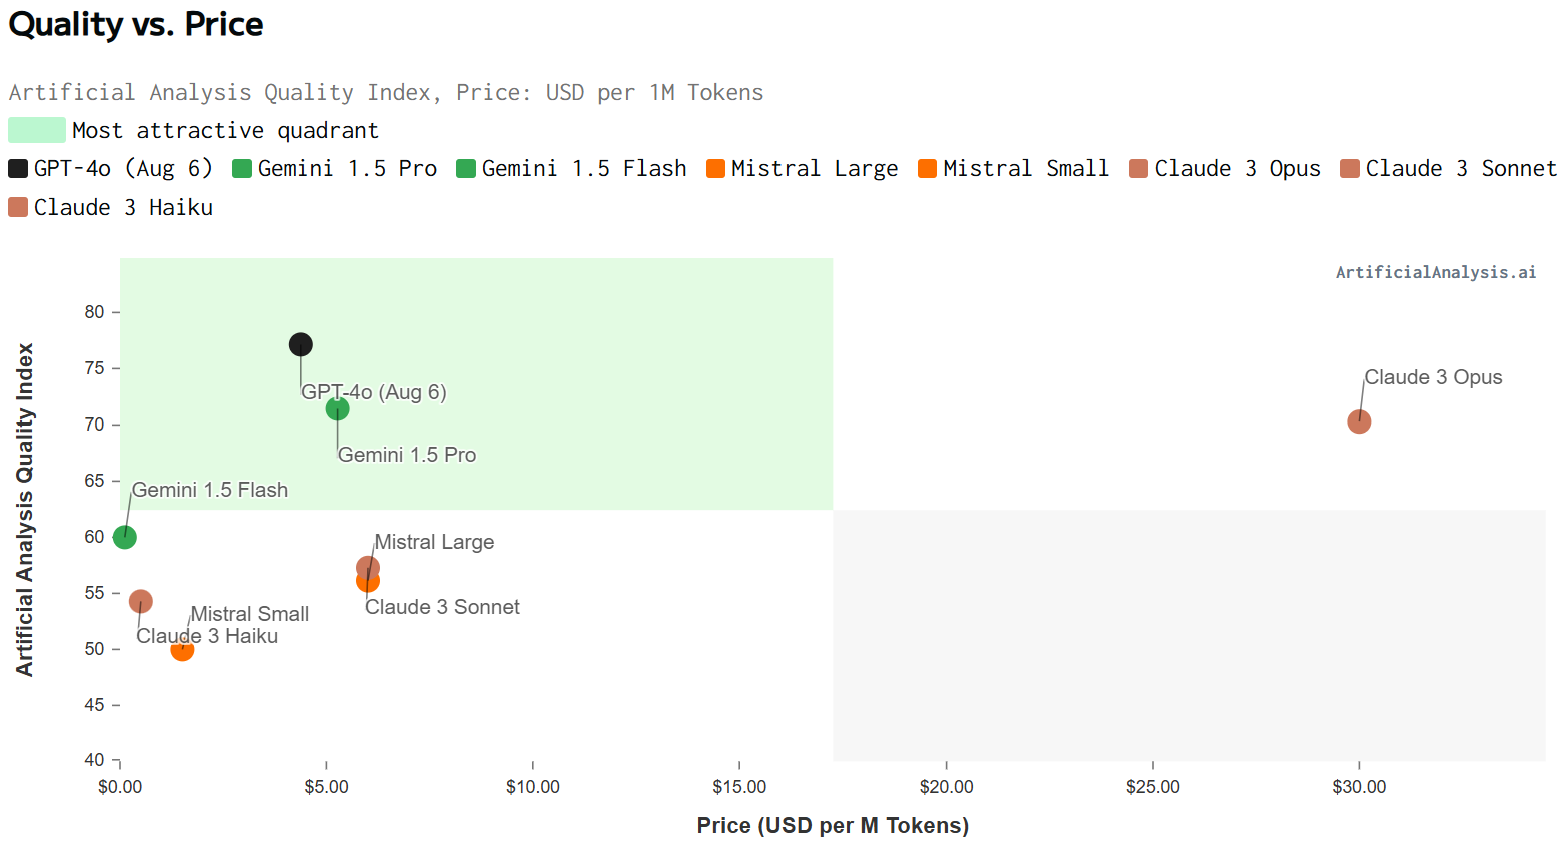
\includegraphics[width=0.9\textwidth]{figuras/capitulo6/quality_price.png}
\caption{Gráfico comparativa calidad contra precio. \citep{artificialanalysis}}
\label{fig:quality_price}
\end{figure}

\subsection{Modelo Embedder}

Este modelo es el encargado de transformar los fragmentos del documento en vectores o embeddings. Este modelo es de alta importancia en el proceso ya que será el que defina la similitud entre los textos. Por tanto es crucial para la recuperación de la información necesaria para dar una respuesta.

El modelo embedder ha sido text-embedding-3-small con posición 59 en el leaderboard de huggingface \citep{leadhugging}. Se ha usado este modelo por ser el mejor calidad/precio disponible en Azure OpenAI. Como se puede ver en la figura \ref{fig:emb_quality} mejora al anterior model ada v2 y se puede ver en la tabla \ref{tab:pricing} como reduce su precio. Por estas dos razones es el modelo seleccionado para el sistema RAG creado.

\begin{figure}[h]
\centering
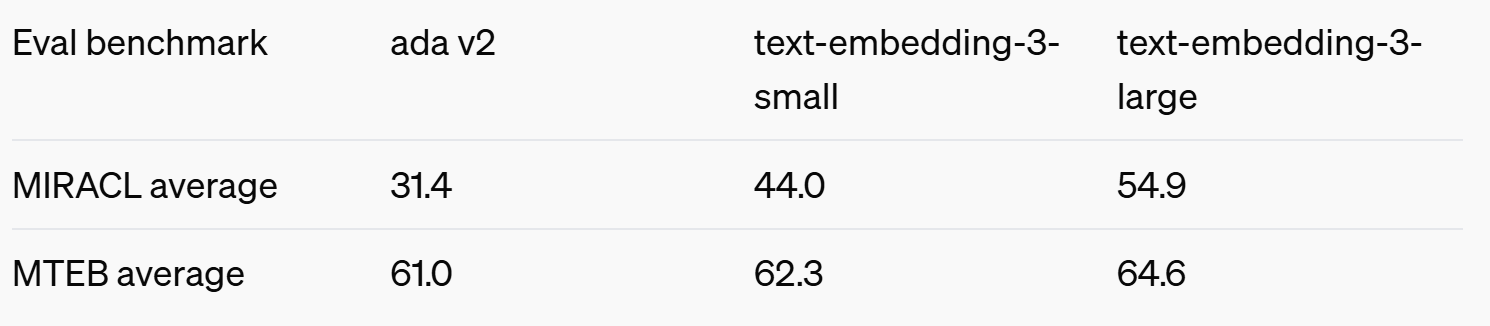
\includegraphics[width=0.9\textwidth]{figuras/capitulo6/emb_quality.png}
\caption{Gráfico calidad embeddings OpenAI \citep{openai}}
\label{fig:emb_quality}
\end{figure}

\begin{table}[h]
\centering
\begin{tabular}{|c|c|}
\hline
\textbf{Model} & \textbf{Pricing} \\ \hline
text-embedding-3-small & \$0.020 / 1M tokens \\ \hline
text-embedding-3-large & \$0.130 / 1M tokens \\ \hline
ada v2 & \$0.100 / 1M tokens \\ \hline
\end{tabular}
\caption{Precio de los embeddings de OpenAI \citep{openai}}
\label{tab:pricing}
\end{table}


\section{Análisis del Documento: Constitución Española}

\subsection{Estructura del Documento}

La \textbf{Constitución Española} es el documento fundamental que establece el marco legal y político de España. Fue ratificada en 1978 y es el texto supremo que rige los derechos, deberes y la organización de las instituciones del país. El documento está dividido en varios títulos que abordan aspectos clave del sistema político, económico y social de España. Se compone de una introducción (Preámbulo) y 10 títulos, además de disposiciones adicionales, transitorias, derogatorias y finales.

\begin{itemize}
    \item \textbf{Preámbulo}: Establece los principios y objetivos fundamentales de la Constitución, como la justicia, la libertad, la democracia, la protección de los derechos humanos, el progreso social y la promoción de la paz y la cooperación internacional.
    \item \textbf{Títulos}:
    \begin{itemize}
        \item \textbf{Título Preliminar}: Define a España como un Estado social y democrático de derecho y establece la soberanía nacional y la forma política del Estado, que es la monarquía parlamentaria.
        \item \textbf{Título I}: Regula los derechos y deberes fundamentales, dividiéndose en varios capítulos que incluyen los derechos de los españoles y los extranjeros, así como las libertades y derechos fundamentales.
        \item \textbf{Título II}: Describe la Corona y las funciones del Rey como jefe de Estado.
        \item \textbf{Títulos III a V}: Tratan sobre las Cortes Generales, el Gobierno y las relaciones entre ambos poderes.
        \item \textbf{Título VI}: Regula el poder judicial.
        \item \textbf{Títulos VII a X}: Abordan la economía y hacienda, la organización territorial del Estado, el Tribunal Constitucional y la reforma constitucional.
    \end{itemize}
\end{itemize}

\subsection{Relevancia para el Sistema RAG}

El \textbf{sistema RAG (Retrieval-Augmented Generation)} que se propone desarrollar utilizará este documento como base de conocimiento para responder preguntas relacionadas con la Constitución Española. Debido a su estructura bien definida y la clara división de temas, es posible fragmentar el documento en secciones más manejables que puedan ser recuperadas de manera eficiente.

\subsection{Formato del documento}

El documento se encuentra tanto en formato PDF como en formato XML. En el formato XML se puede acceder a cada uno de los artículos de la constitución por separado. Se muestra un ejemplo a continuación:

\begin{verbatim}
</div>
<p class="linkSubir"><a href="https://www.boe.es/buscar/act.php?
id=BOE-A-1978-31229&amp;p=20240217&amp;tn=1#top">Subir</a></p>
<hr class="bloque">
<div class="bloque" id="a3">
  <p class="bloque">[Bloque 5: #a3]</p>
  <form action="https://www.boe.es/buscar/act.php?id=BOE-A-1978-31229&amp;
  p=20240217&amp;tn=1#" method="get">
    <input type="hidden" value="BOE-A-1978-31229" name="id">
    <input type="hidden" value="5" name="tn">
    <input type="hidden" value="a3" name="bj">
    <input id="btn_jur_a3" type="submit">
    <label for="btn_jur_a3" title="Jurisprudencia">
      <span class="fuera">Jurisprudencia</span>
    </label>
  </form>
  <h5 class="articulo">Artículo 3</h5>
  <p class="parrafo">1. El castellano es la lengua española oficial del Estado. 
  Todos los españoles tienen el deber de conocerla y el derecho a usarla.</p>
  <p class="parrafo">2. Las demás lenguas españolas serán también oficiales en las 
  respectivas Comunidades Autónomas de acuerdo con sus Estatutos.</p>
  <p class="parrafo">3. La riqueza de las distintas modalidades lingüísticas de 
  España es un patrimonio cultural que será objeto de especial respeto y protección.</p>
</div>
\end{verbatim}

\section{Chunkerización del Documento}

La chunkerización es un proceso crucial en la creación de sistemas de Recuperación Aumentada por Generación (RAG, por sus siglas en inglés). En este capítulo, se describe cómo se realiza la chunkerización del documento de la Constitución Española para mejorar la eficiencia en la recuperación de la información. Utilizamos diferentes estrategias de chunkerización que se adaptan a la naturaleza del texto y el caso de uso. Para implementar estas estrategias, utilizamos la librería \texttt{LangChain}, que ofrece una serie de herramientas avanzadas para manejar documentos de gran tamaño.

\section{Estrategias de Chunkerización}

La chunkerización del documento implica dividir el texto en fragmentos más pequeños y manejables (chunks). Esto mejora la precisión de la recuperación de información al asegurar que los fragmentos estén centrados en temas específicos. A continuación, se explican las tres estrategias de chunkerización empleadas:

\subsection{Character Text Splitter}
El \textit{Character Text Splitter} es una de las técnicas básicas de chunkerización. Divide el texto en fragmentos basándose en un número fijo de caracteres, lo que asegura que los fragmentos resultantes tengan un tamaño consistente. Esta técnica es útil cuando se requiere dividir grandes bloques de texto de manera uniforme, pero no considera la semántica ni la estructura del texto.

Para esta estrategia, definimos tamaños de chunk de 200, 300 y 400 caracteres, con un pequeño solapamiento entre los fragmentos (10 \% del tamaño del chunk), lo que permite preservar el contexto cuando se fragmenta el documento. Este método es sencillo y eficiente para manejar grandes volúmenes de datos.

\subsection{Recursive Character Text Splitter}
El \textit{Recursive Character Text Splitter} es una versión más avanzada del \textit{Character Text Splitter}. Además de dividir el texto basándose en el número de caracteres, este enfoque aplica un análisis recursivo, respetando la estructura del documento al intentar evitar cortar palabras o frases importantes. De esta manera, los fragmentos generados tienen mayor coherencia interna y preservan mejor el contexto semántico, lo que mejora las respuestas generadas en los sistemas RAG.

Al igual que con el splitter básico, se utilizan tamaños de chunk de 200, 300 y 400 caracteres, pero con el beneficio añadido de que los fragmentos resultan más naturales y mejor alineados con las divisiones lógicas del texto.

\subsection{Chunkerización personalizada (Spanish Article Splitter)}
El \textit{Spanish Article Splitter} ha sido desarrollado específicamente para chunkerizar documentos legales en español, como la Constitución Española. Este splitter aprovecha la estructura inherente del documento en XML, basada en artículos, para realizar la chunkerización. Utilizando técnicas de procesamiento de HTML, el splitter identifica los artículos individuales y los divide en fragmentos de texto correspondientes. Cada artículo es tratado como un fragmento separado, preservando su integridad semántica.

Este splitter es particularmente útil en textos legales, donde cada artículo puede ser considerado una unidad independiente y completa de información. Para documentos como la Constitución Española, esta técnica asegura que los fragmentos de texto sean coherentes y estén alineados con la estructura legal del documento.

El pseudocódigo del algoritmo desarrollado se encuentra en el algoritmo \ref{alg:SpanishArticleSplitter}.


\begin{algorithm}
\caption{SpanishArticleSplitter}\label{alg:SpanishArticleSplitter}
\textbf{Entrada:} Ruta del archivo HTML (\textit{file\_path}) \;
\textbf{Salida:} Lista de documentos divididos por artículos (\textit{documents}) \;

Abrir el archivo en la ruta especificada (\textit{file\_path}) y leer su contenido como HTML\;
Parsear el contenido HTML utilizando un parser compatible con HTML\;
Inicializar una lista vacía para almacenar los documentos (\textit{documents})\;
Encontrar todos los elementos de encabezado \texttt{<h5>} con la clase \texttt{articulo}\;
\For{cada \texttt{<h5>} encontrado}{
    Encontrar el \texttt{<div>} que contiene el artículo asociado\;
    Extraer el nombre del artículo desde el texto del encabezado \texttt{<h5>}\;
    Inicializar una lista vacía para los párrafos del artículo\;
    \For{cada párrafo \texttt{<p>} dentro del \texttt{<div>}}{
        \If{el texto del párrafo no contiene \texttt{"Bloque"}}{
            Agregar el texto del párrafo a la lista\;
        }
    }
    Unir todos los párrafos para formar el texto completo del artículo\;
    Crear un diccionario de metadatos con nombre del artículo, nombre del archivo y fuente del archivo\;
    Crear un documento con el texto del artículo y los metadatos\;
    Agregar el documento a la lista \textit{documents}\;
}
Retornar la lista de documentos \textit{documents}\;
\end{algorithm}

\subsection{Librería LangChain}
La librería usada para esta tarea ha sido \texttt{LangChain}. Proporciona una plataforma robusta para la manipulación y chunkerización de documentos. Permite el uso de diferentes tipos de splitters para dividir el texto según las necesidades del usuario. En este caso, se emplearon tanto splitters estándar como personalizados. La flexibilidad de \texttt{LangChain} facilita la integración de diferentes enfoques, desde la división básica de texto por caracteres hasta estrategias más complejas como el \textit{Spanish Article Splitter}.

LangChain también facilita el procesamiento de diferentes formatos de documentos (como PDF y HTML) y su posterior transformación en fragmentos manejables para mejorar la eficiencia en los procesos de recuperación y generación de texto.\\

En total se obtienen 7 formas de fragmentar el documento que deberán ser evaluadas.


\section{Evaluación del sistema RAG}

Para evaluar la efectividad de la chunkerización en el sistema RAG creado, se utilizó un proceso exhaustivo que involucró la generación y evaluación de preguntas basadas en los fragmentos generados de la Constitución Española. Este proceso de evaluación fue realizado utilizando la librería \texttt{LlamaIndex}, que permitió automatizar tanto la generación de preguntas como la medición de métricas clave para determinar la calidad de las respuestas generadas.

Es importante puntualizar que el número de chunks devueltos por el sistema RAG de cara a su evaluación ha sido de 2 chunks.

\subsection{Generación de Preguntas}

El primer paso consistió en generar un conjunto de preguntas para evaluar la precisión y relevancia de las respuestas proporcionadas por el sistema. Para ello, se utilizó el modelo GPT-3.5-turbo, que empleó un \textit{prompt} diseñado para generar preguntas en español a partir de fragmentos de texto extraídos de los documentos chunkerizados. Este conjunto de preguntas se almacenó en un archivo CSV para su posterior uso en la evaluación.

Se usó el siguiente prompt para la generación de preguntas:

\begin{verbatim}
Context information is below.
---------------------
{context_str}
---------------------
Given the context information and not prior knowledge,
generate only questions based on the below query.
Generate the questions in Spanish.
{query_str}
\end{verbatim}

\begin{table}[h]
\centering
\begin{tabular}{|c|}
\hline
\textbf{Questions} \\ \hline
¿Cuáles son los valores superiores del ordenamiento jurídico en España? \\ \hline
¿En quién reside la soberanía nacional en España? \\ \hline
¿Cuál es la forma política del Estado español? \\ \hline
¿Cómo se define a España en términos de su Estado? \\ \hline
¿Cuáles son los principios fundamentales de España como Estado? \\ \hline
¿Cuál es el sistema político de España? \\ \hline
¿Qué poderes emanan del pueblo español? \\ \hline
¿Qué tipo de monarquía tiene España? \\ \hline
... \\ \hline
\end{tabular}
\caption{Ejemplo de preguntas generadas}
\label{tab:questions}
\end{table}


\subsection{Métricas de Evaluación}

Las métricas de evaluación clave empleadas en este proceso se centran en tres aspectos fundamentales para sistemas RAG: fidelidad, relevancia de la respuesta, relevancia del contexto y tiempo de respuesta. Estas métricas se calcularon utilizando el modelo GPT-4o (\textbf{modelo juez}), que permitió evaluar de manera automática la calidad de las respuestas generadas para cada pregunta.

\begin{itemize}
    \item \textbf{Fidelidad (FP)}: Mide hasta qué punto las respuestas generadas están respaldadas por el contexto proporcionado. Es decir, se asegura de que las afirmaciones hechas en las respuestas sean consistentes con la información del documento original, minimizando la aparición de alucinaciones. En la implementación de LlamaIndex el resultado será True o False.
    \item \textbf{Relevancia de la Respuesta (RP)}: Evalúa si la respuesta aborda directamente la pregunta formulada. Este criterio no solo considera la factualidad, sino también si la respuesta es completa y libre de información redundante o innecesaria. En la implementación de LlamaIndex el resultado será True o False.
    \item \textbf{Relevancia del Contexto (RCP)}: Mide cuán relevante es el contexto recuperado para responder la pregunta. Un buen contexto debe contener únicamente la información necesaria para proporcionar una respuesta precisa, sin añadir detalles irrelevantes que puedan afectar la calidad de la generación de texto.
    \item \textbf{Tiempo de respuesta (TRP)}: El tiempo en el que el sistema RAG completo da una respuesta a la pregunta del usuario.
\end{itemize}

Cabe recalcar que ninguna de las métricas usadas necesita la respuesta verdadera a la pregunta ya que analizan la respuesta en base al contexto (los chunks) aportado.

En la tabla \ref{tab:evaluation1} puede verse un ejemplo de error con la respuesta, sin embargo todas las métricas cumplen su función.

\begin{itemize}
    \item \textbf{Fidelidad}: El resultado es True ya que no hay alucinación en la respuesta. El Agente LLM no tiene en el contexto la información que el usuario solicita por lo que la respuesta es correcta al responder que no puede responder.
    \item \textbf{Relevancia de la Respuesta}: Esta métrica mide la relevancia de la respuesta a la pregunta. En otras palabras si responde la pregunta del usuario. El resultado es True, ya que responde que no puede responder con la información que tiene, pero responde a la pregunta formulada.
    \item \textbf{Relevancia del Contexto}: En esta métrica si podemos comprobar que el contexto no es el adecuado para responder a la pregunta y el modelo juez aporta la explicación de esta métrica.
\end{itemize}

\begin{table}[h]
\centering
\begin{tabular}{|p{4cm}|p{11cm}|}
\hline
\textbf{Field} & \textbf{Content} \\ \hline
\textbf{Question} & ¿Cuál es el contenido del artículo 28 de la Constitución Española? \\ \hline
\textbf{Response} & El contenido del artículo 28 de la Constitución Española no se encuentra proporcionado en el contexto dado. \\ \hline
\textbf{Context 1} & 
\textbf{Article Name:} Artículo 53 \newline 
\textbf{Text:} Los derechos y libertades reconocidos en el Capítulo segundo del presente Título vinculan a todos los poderes públicos... \newline
\textbf{Source:} ../data/Constitución Española/BOE-A-1978-31229 Constitución Española.html
\\ \hline
\textbf{Context 2} & 
\textbf{Article Name:} Artículo 20 \newline
\textbf{Text:} Se reconocen y protegen los derechos: \newline
a) A expresar y difundir libremente los pensamientos, ideas y opiniones mediante la palabra, el escrito o cualquier otro medio... \newline
\textbf{Source:} ../data/Constitución Española/BOE-A-1978-31229 Constitución Española.html
\\ \hline
\textbf{Faithfulness} & True \\ \hline
\textbf{Relevancy} & True \\ \hline
\textbf{Context Relevancy Score} & 0.125 \\ \hline
\textbf{Context Relevancy Feedback} & 
\textbf{Feedback:} \newline
- The context is related to the Spanish Constitution but does not specifically match Article 28. \newline
- **Score:** 0.5/2 \newline
- The context does not provide the specific content needed to answer the query. \newline
- **Final Score:** 0.5
\\ \hline
\textbf{Response Time} & 1.253065586090088 seconds \\ \hline
\end{tabular}
\caption{Ejemplo evaluación pregunta 1}
\label{tab:evaluation1}
\end{table}

\begin{table}[h]
\centering
\begin{tabular}{|p{4cm}|p{11cm}|}
\hline
\textbf{Field} & \textbf{Content} \\ \hline
\textbf{Question} & ¿Cuál es el objetivo de la educación según los principios constitucionales? \\ \hline
\textbf{Response} & El objetivo de la educación según los principios constitucionales es el pleno desarrollo de la personalidad humana en el respeto a los principios democráticos de convivencia y a los derechos y libertades fundamentales. \\ \hline
\textbf{Context 1} & 
\textbf{Article Name:} Artículo 27 \newline 
\textbf{Text:} Todos tienen el derecho a la educación. Se reconoce la libertad de enseñanza... \newline
\textbf{Source:} ../data/Constitución Española/BOE-A-1978-31229 Constitución Española.html
\\ \hline
\textbf{Context 2} & 
\textbf{Article Name:} Artículo 9 \newline
\textbf{Text:} Los ciudadanos y los poderes públicos están sujetos a la Constitución... \newline
\textbf{Source:} ../data/Constitución Española/BOE-A-1978-31229 Constitución Española.html
\\ \hline
\textbf{Faithfulness} & True \\ \hline
\textbf{Relevancy} & True \\ \hline
\textbf{Context Relevancy Score} & 1.0 \\ \hline
\textbf{Context Relevancy Feedback} & 
\textbf{Feedback:} \newline
- The retrieved context directly addresses the query about the objective of education. \newline
- **Score:** 2/2 \newline
- The context can be used exclusively to fully answer the query. \newline
- **Final Score:** 4.0
\\ \hline
\textbf{Response Time} & 2.0108368396759033 seconds \\ \hline
\end{tabular}
\caption{Ejemplo evaluación pregunta 2}
\label{tab:evaluation12}
\end{table}

\subsection{Evaluación}

Se creó una base de datos vectorial sobre chroma utilizando los grupos de documentos chunkerizados anteriormente, y para cada pregunta y grupo de chunks (cada metodología de chunkerización descrita), el sistema calculó las métricas de fidelidad, relevancia de la respuesta, relevancia del contexto y tiempo de respuesta.

El proceso de evaluación se llevó a cabo mediante la generación de respuestas automáticas a las preguntas formuladas. Se calculó el promedio de las métricas para cada metodología de chunks. Finalmente, los resultados de las métricas se almacenaron en un archivo JSON para su análisis posterior.

\subsection{Resultados}

Se presentan los resultados de la evaluación de diferentes técnicas de chunkerización aplicadas al sistema RAG. A continuación, se describen los resultados obtenidos para cada estrategia de chunkerización (véase tabla \ref{tab:chunk_results} y la figura \ref{fig:chunk_plot}):

\begin{itemize}
    \item \textbf{Spanish Article Splitter}: Esta estrategia produjo un tiempo de respuesta promedio de 1.56 segundos, con una fidelidad promedio de 0.94, una relevancia promedio de 0.94 y una relevancia del contexto de 0.86. Estos resultados muestran que este splitter mantiene un alto nivel de precisión en las respuestas y una relevancia adecuada del contexto, aunque el tiempo de respuesta es ligeramente superior a otras estrategias.
    
    \item \textbf{Character Splitter (400 caracteres)}: El tiempo de respuesta promedio fue de 1.52 segundos, con una fidelidad de 0.95, relevancia de 0.91 y relevancia del contexto de 0.72. Esta estrategia proporcionó un excelente balance entre fidelidad y relevancia, aunque la relevancia del contexto es menor en comparación con el splitter basado en artículos.
    
    \item \textbf{Recursive Character Splitter (400 caracteres)}: Este splitter alcanzó un tiempo de respuesta promedio de 1.50 segundos, con una fidelidad de 0.93, relevancia de 0.87 y relevancia del contexto de 0.69. Aunque la relevancia del contexto es menor, esta técnica ofrece un buen equilibrio entre tiempos de respuesta y precisión.
    
    \item \textbf{Recursive Character Splitter (200 caracteres)}: El tiempo de respuesta promedio fue el más bajo con 1.43 segundos. La fidelidad promedio fue de 0.95, la relevancia de 0.85 y la relevancia del contexto de 0.65. Aunque presenta buenos tiempos de respuesta, la relevancia del contexto es la más baja entre las estrategias evaluadas.
    
    \item \textbf{Character Splitter (300 caracteres)}: Con un tiempo de respuesta promedio de 1.30 segundos, esta estrategia obtuvo una fidelidad de 0.91, relevancia de 0.83 y relevancia del contexto de 0.67. Aunque el tiempo de respuesta es rápido, las métricas de relevancia están ligeramente por debajo de otras técnicas.
    
    \item \textbf{Recursive Character Splitter (300 caracteres)}: Este splitter alcanzó un tiempo de respuesta promedio de 1.39 segundos, con una fidelidad de 0.94, relevancia de 0.90 y relevancia del contexto de 0.69. Aunque el tiempo de respuesta es mayor que otras técnicas, ofrece un buen compromiso entre precisión y relevancia de las respuestas.
    
    \item \textbf{Character Splitter (200 caracteres)}: El tiempo de respuesta promedio fue de 1.36 segundos, con una fidelidad de 0.91, relevancia de 0.82 y relevancia del contexto de 0.65. Este splitter tuvo uno de los tiempos de respuesta más rápidos, pero mostró una ligera disminución en las métricas de relevancia y contexto.

\end{itemize}

En general, los resultados muestran que la estrategia \textit{Spanish Article Splitter} ofrece las mejores métricas de fidelidad y relevancia, a pesar de un tiempo de respuesta ligeramente superior. Por otro lado, las estrategias basadas en \textit{Character Splitter} y \textit{Recursive Character Splitter} presentan una relación equilibrada entre tiempos de respuesta rápidos y métricas de calidad aceptables, con la versión de 400 caracteres proporcionando el mejor compromiso entre velocidad y precisión.

\begin{table}[h]
\centering
\begin{tabular}{|l|c|c|c|c|}
\hline
\textbf{Chunkerización} & \textbf{TRP (s)} & \textbf{FP} & \textbf{RP} & \textbf{RCP} \\ \hline
\textbf{Spanish Article Splitter} & 1.56 & 0.94 & 0.94 & 0.86 \\ \hline
\textbf{Character Splitter (400 caracteres)} & 1.52 & 0.95 & 0.91 & 0.72 \\ \hline
\textbf{Recursive Character Splitter (400 caracteres)} & 1.50 & 0.93 & 0.87 & 0.69 \\ \hline
\textbf{Recursive Character Splitter (200 caracteres)} & 1.43 & 0.95 & 0.85 & 0.65 \\ \hline
\textbf{Character Splitter (300 caracteres)} & 1.30 & 0.91 & 0.83 & 0.67 \\ \hline
\textbf{Recursive Character Splitter (300 caracteres)} & 1.39 & 0.94 & 0.90 & 0.69 \\ \hline
\textbf{Character Splitter (200 caracteres)} & 1.36 & 0.91 & 0.82 & 0.65 \\ \hline
\end{tabular}
\caption{Resultados de la Evaluación de las Técnicas de Chunkerización}
\label{tab:chunk_results}
\end{table}

\begin{figure}[h]
\centering
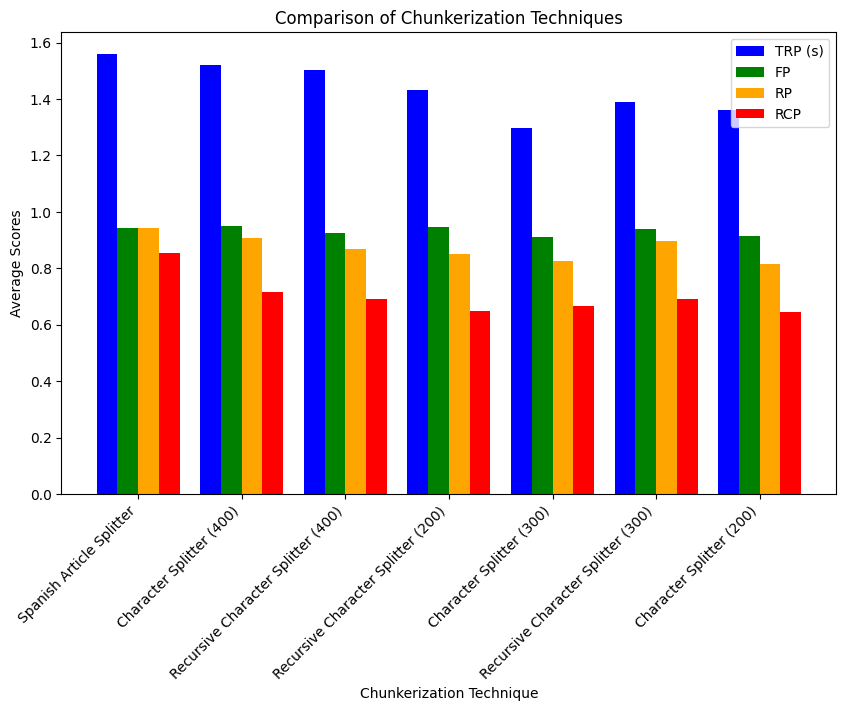
\includegraphics[width=0.6\textwidth]{figuras/capitulo6/score_splitters.png}
\caption{Gráfico comparativo de los splitters evaluados}\label{fig:chunk_plot}
\end{figure}



\section{Creación del agente}

Por último, se ha creado el agente mendiante la librería Langchain usando el splitter personalizado para los artículos de la constitución española. Para ello se ha usado un retriever denso descrito en el capítulo 5. Se ha implementado la arquitectura de la figura \ref{fig:retriever}.

Para que sea más visual (figura \ref{fig:chat1}) y haya una interfaz con la que interactuar con el agente, se ha implementado una app usando la librería Streamlit. En esta interfaz web se pueden hacer preguntas de todo tipo. A continuación se muestran ejemplos de preguntas sobre la interfaz, donde a la vez de ser visualmente más agradable también se muestra un desplegable con el contexto (figura \ref{fig:chat2}) utilizado para responder a la pregunta.

\begin{figure}[h]
\centering
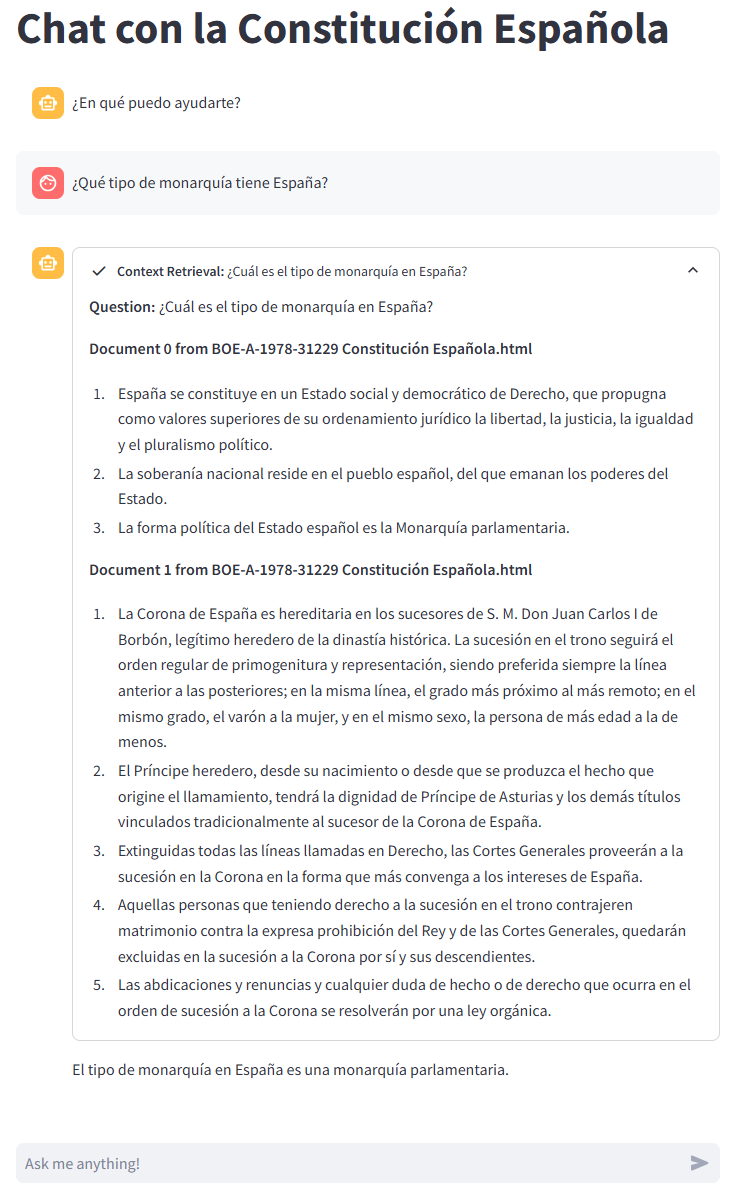
\includegraphics[width=0.7\textwidth]{figuras/capitulo6/chat2exp.png}
\caption{Ejemplo de pregunta en Chat con contexto expandido}\label{fig:chat2}
\end{figure}

\newpage

\begin{figure}[h]
\centering

\includegraphics[width=0.7\textwidth]{figuras/capitulo6/chat1.png}
\caption{Ejemplo de pregunta en Chat}\label{fig:chat1}
\end{figure}

\subsection{Diagrama Arquitectura}

El diagrama de arquitectura de la app desarrollada es el siguiente:

\begin{figure}[h]
\centering
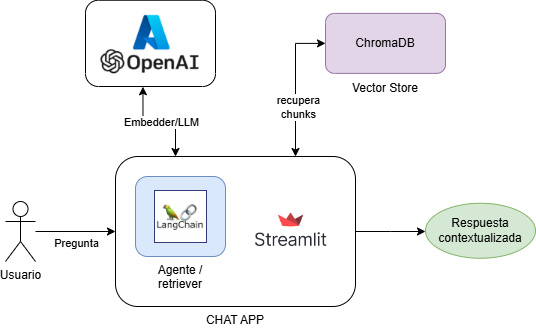
\includegraphics[width=0.7\textwidth]{figuras/capitulo6/arquitectura.png}
\caption{Arquitectura desarrollada}\label{fig:arquitectura}
\end{figure}

En el diagrama se puede ver como las consultas al LLM y al embedder se hacen a través de Azure OpenAI, el vector store utilizado es una instancia de ChromaDB, el agente (retriever) se desarrolla usando el framework Langchain y finalmente la interfaz se ha creado con Streamlit.

\section{Conclusión}

Este capítulo describe la implementación de un sistema RAG para responder preguntas sobre la Constitución Española. Se utilizan modelos LLM como GPT-4o para la evaluación y GPT-3.5-Turbo para generar respuestas, junto con un modelo de embeddings para procesar el texto. Se analizan y prueban varias estrategias de chunkerización del documento, como Character Text Splitter y Spanish Article Splitter, optimizando la recuperación de información.

La evaluación de las técnicas demuestra que el Spanish Article Splitter ofrece la mejor precisión y relevancia del contexto, aunque con un ligero aumento en el tiempo de respuesta. Finalmente, se implementa una interfaz web interactiva para facilitar el uso del sistema, mostrando cómo se puede automatizar la consulta legal de manera eficiente.


